% ============================================================
% LLaVA-1.6 replication -- ADDITION TO main_final.tex, kept separate for review.
%
% Suggested placement:
%   * Section "Replication on LLaVA-1.6 with task-trained dictionaries" goes
%     after the Gemma 3 section (Section~\ref{sec:gemma}) and before the
%     Discussion.
%   * The appendix section goes after Appendix~\ref{app:gemma}.
%   * Figures: llava16_fig1_knockout_landscape, llava16_fig_decomposition,
%     llava16_fig6_budget_distribution, llava16_fig8a_ablation_vs_knockout,
%     llava16_fig8b_recovered_share, llava16_fig_single_layer, in
%     paper_figures/ (PNG + PDF).
%   * Bibliography entries to append to refs.bib are at the end of this file.
%   * Suggested changes to the abstract, the Limitations paragraph and
%     Availability are given as comments at the end. The Limitations sentence
%     is a COMBINED replacement: it also carries the Gemma 3 addition's
%     suggestion, since both edit the same sentence.
%
% Every number below is read from committed artifacts of the vlm-flow-probe
% repo (output/experiments/llava16_*; see docs/llava16_replication.md there for
% the run log and the decision record). All 53 conditions share the same
% first-256 validation questions in the same order (SHA-1 a74b46cc..., verified
% by the analysis), so paired statements hold as in the LLaVA-1.5 runs.
%
% One scale caveat, stated in the appendix and worth knowing while reading the
% tables: absolute margins are not comparable between LLaVA-1.5 and LLaVA-1.6,
% because the two checkpoints tokenise the scored answer string differently.
% R = A/K is a ratio and is unaffected.
% ============================================================

% ------------------------------------------------------------
% Self-compiling guard.  If this file is compiled on its own (Overleaf's
% "main document"), it loads a class and opens the document environment; if it
% is \input into main_final.tex, the class is already loaded and the whole
% block is skipped.  Keep it -- without it a solo compile produces no PDF
% ("the document environment contains no content").
% ------------------------------------------------------------
\expandafter\ifx\csname @classoptionslist\endcsname\relax
  \documentclass[11pt,a4paper]{article}
  \usepackage[T1]{fontenc}
  \usepackage{lmodern}
  \usepackage[margin=2.5cm]{geometry}
  \usepackage{amsmath,amssymb}
  \usepackage{graphicx}
  \usepackage{booktabs}
  \usepackage{multirow}
  \usepackage{array}
  \usepackage{hyperref}
  \usepackage{xcolor}
  \usepackage{microtype}
  \usepackage{parskip}
  \usepackage[round]{natbib}
  \graphicspath{{paper_figures/}{figures/}}
  \begin{document}
  \newcommand{\llavasixstandalone}{}
\fi

\section{Replication on LLaVA-1.6 with task-trained dictionaries}
\label{sec:llava16}

The Gemma~3 replication changed the model, the dictionaries, the hook site and
the answer convention at once, and failed on all three preconditions. This one
changes as little as it is possible to change and still have a different model.
LLaVA-1.6 \citep{llavanext} keeps LLaVA-1.5's Vicuna-7B decoder, and we keep the
prompt, the data, the metric, the SAE recipe and the condition matrix. What
differs is the vision front-end: AnyRes tiling turns the same $224\times224$
CLEVR-Lite image into 1{,}176 image tokens instead of 576. The question is
whether the calibration survives a doubled visual context in front of the same
language model.

It does not, and every precondition holds while it fails. That is the point of
reporting it.

\paragraph{Setup.} \texttt{llava-v1.6-vicuna-7b}: the same 32-layer,
$d_{\text{model}} = 4096$ Vicuna-7B decoder as LLaVA-1.5 \citep{llava15}, behind
an AnyRes vision front-end that encodes a base view and unpadded high-resolution
tiles separately and joins tile rows with a learned newline embedding. For a
square CLEVR-Lite image the processor selects a $336\times672$ pinpoint and
emits $576 + 576 + 24 = 1{,}176$ image tokens, a 1{,}235-token prompt against
636. Dictionaries are trained here, on this model's own activations, with the
LLaVA-1.5 recipe unchanged: ReLU with an $L_1$ penalty, 32{,}768 features at the
attention output, question positions of the training split. We train all 32
layers rather than the six of the original study, so the single-layer landscape
covers the whole stack. Everything else is held fixed: CLEVR-Lite, the same
validation split and the same first-256 evaluation questions, the margin
$\log P(\text{true}) - \log P(\text{false})$ with per-token normalisation,
gradient$\times$activation selection with $k = 200$ per layer,
\texttt{replace}-mode ablation, activation-matched controls, and the condition
matrix.

\paragraph{The three preconditions hold.} The dictionaries fit the site:
explained variance runs 0.9989--0.9999 across all 32 layers
(Table~\ref{tab:llava16-sae}), against 0.9985--0.9998 for the LLaVA-1.5
dictionaries in Table~\ref{tab:sae} and 0.67--0.95 for Gemma~Scope~2's, and
under 0.2\% of features are dead at every span layer (layer~0 is 79\% dead, as
it was 74\% dead on LLaVA-1.5, and no layer the ablation analysis uses exceeds
15\%). \texttt{replace}-mode pass-through
is therefore usable and was checked before any ablation was interpreted: with
nothing ablated, substituting the reconstruction at every question position of
layers 10--14 moves the margin by $+0.0078$, and by at most that over any nested
sub-span (Appendix~\ref{app:llava16}), against $+0.0011$ on LLaVA-1.5 and
$+1.56$ on Gemma. The margin is far from saturation: the unmodified model puts
the true option at $-9.73$ and the false one at $-16.53$, a margin of 6.80, with
forced-choice accuracy 0.934 and generation accuracy 0.672 on the evaluation
set. And the features act on the pathway the knockout severs --- with
Image$\rightarrow$Question blocked at all 32 layers the model sits at chance
(margin $+0.13$, forced-choice accuracy 0.484, generation accuracy 0.000), and
ablating the span's 1{,}000 selected features on top of that moves the margin by
$+0.03$; it lowers both options by about four nats together rather than
separating them.

\paragraph{The landscape is LLaVA-1.5's.} Figure~\ref{fig:llava16-landscape}
gives the sweep over all 32 layers, on the 7{,}186 of 7{,}790 validation
questions the unmodified model answers correctly (7{,}084 for LLaVA-1.5).
Image$\rightarrow$Question transfer concentrates at layer~0 (margin drop 1.944),
then 11 (1.512) and 14 (1.313), then a weaker late group at 19 (0.639), 17
(0.510) and 10 (0.464); 11 of the 32 layers are inhibitory, none strongly.
The top-three set is $\{0, 11, 14\}$ --- identical to LLaVA-1.5's. Applying the
same span rule as the original study, the contiguous band holding the strongest
sites other than layer~0 with inhibitory members retained, gives \emph{layers
10--14}: the same span, the same concentrated layer (11), and the same
sign-inconsistent member (13, knockout $-0.183$). The condition matrix generated
from that span is field-for-field identical to the published one. Doubling the
visual context does not move where cross-modal transfer happens.
Image$\rightarrow$Last, by contrast, peaks later than on LLaVA-1.5, at layers 19
(0.558), 17 (0.411) and 14 (0.343).

\begin{figure}[t]
  \centering
  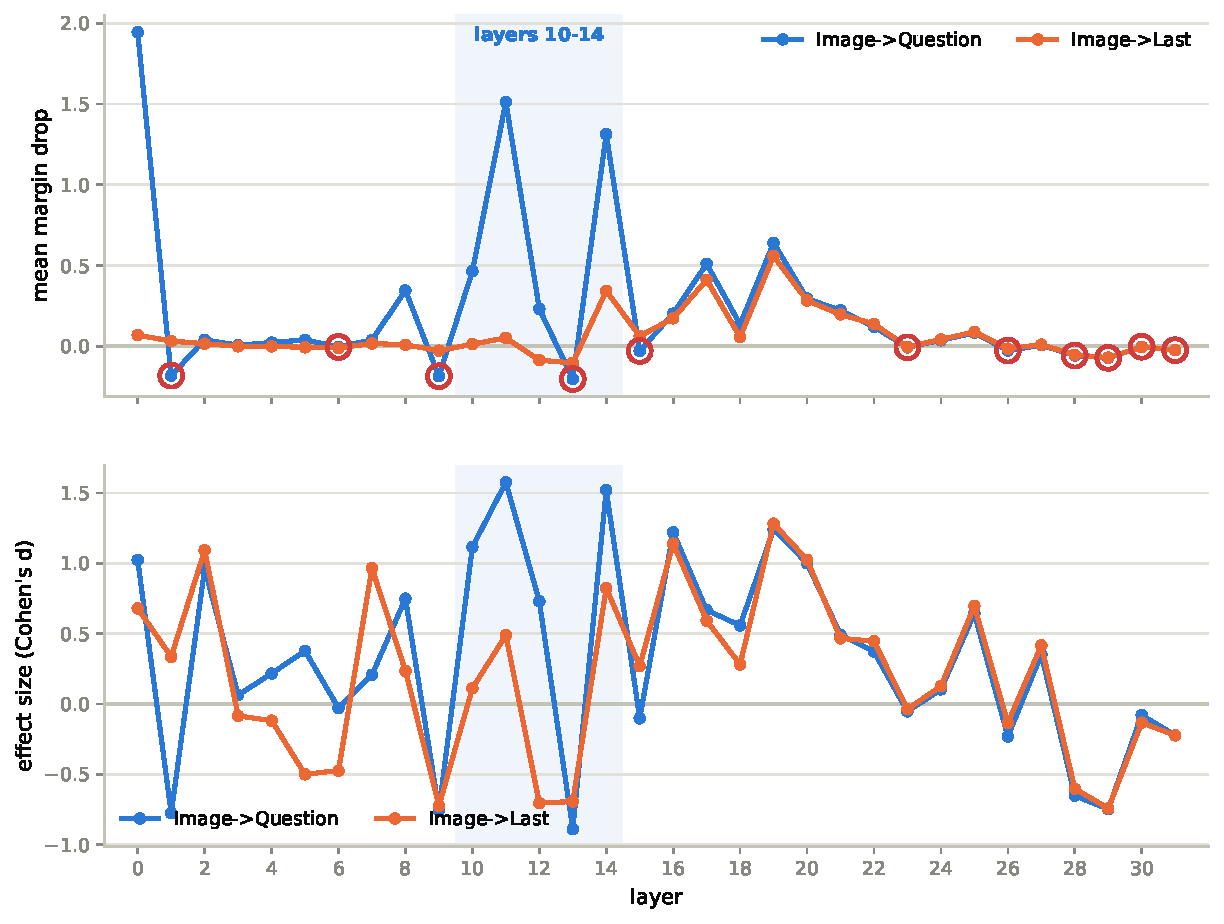
\includegraphics[width=\textwidth]{llava16_fig1_knockout_landscape}
  \caption{\textbf{LLaVA-1.6 knockout landscape.} Mean margin drop (top) and
  Cohen's $d$ (bottom) from blocking Image$\rightarrow$Question (blue) and
  Image$\rightarrow$Last (orange) attention at each of the 32 decoder layers,
  $n = 7{,}186$. Ringed points are inhibitory. The shaded band marks layers
  10--14, fixed as the analysis span from this sweep --- the same band the
  published LLaVA-1.5 study used, chosen by the same rule.}
  \label{fig:llava16-landscape}
\end{figure}

\paragraph{The recovered share does not transfer.} Over the full span, ablation
recovers $R = 93.6\%$ of the severed pathway (95\% CI $[89.0, 98.5]$; $A = 3.64$
against $K = 3.89$), where LLaVA-1.5 gives 72.6\% (95\% CI $[69.6, 75.8]$).
Pooled over the nested spans the figure is 120.6\% (95\% CI $[115.7, 125.7]$),
because at short spans ablation \emph{exceeds} the knockout ceiling: 138.1\% at
$\{14\}$, 194.5\% at $\{13,14\}$, 183.6\% at $\{12,13,14\}$, falling to 93.7\%
and 93.6\% at four and five layers (Table~\ref{tab:llava16-spans},
Figure~\ref{fig:llava16-spans}). As on LLaVA-1.5, no single value lies inside
every interval, so $R$ is not a fixed share on either model. Unlike LLaVA-1.5,
it trends: the slope is $-0.190$ per layer (95\% CI $[-0.212, -0.169]$), where
the published run gives $-0.010$ (95\% CI $[-0.024, +0.003]$), a slope
indistinguishable from zero. The two nested curves make the same point without
the ratio: ablation grows at 1.766 per layer against the knockout's 0.762, a
slope ratio of 2.318, where LLaVA-1.5 gives 0.193 and 0.269, a ratio of 0.718.
On LLaVA-1.5 the ablation curve is the shallower of the two; here it is steeper
by more than a factor of two.

An intervention above the ceiling at the same locus was, on Gemma, the signature
of ablation acting off the pathway. Here the isolation condition rules that
reading out, and a different one fits the numbers: a single-layer knockout is
cheap for the model to route around, because it can re-read the image at any of
the other 31 layers, so $K$ is small at short spans; the ablation removes content
from the residual stream that later layers cannot restore by re-reading. Severing
five layers at once is much harder to route around --- $K$ jumps from 1.54 at
three layers to 3.59 at four --- and there the two interventions come back into
line. We do not test this directly, and it predicts a span width at which the
curves cross that this design does not measure.

\paragraph{What does transfer.} The qualitative account survives intact. Where a
budget is allocated still matters more than its size: 200 features spread over
the five span layers drop the margin by 1.359 against 0.695 concentrated at
layer~11, a factor of 1.96, where LLaVA-1.5 reports roughly three
(Figure~\ref{fig:llava16-budget}); the concentrated curve is again close to flat
in $k$, moving only from 0.517 at $k = 100$ to 0.774 at $k = 400$ and falling
back to 0.579 at $k = 800$. The redundancy signature is the same: leave-one-out
marginal contributions are far below the standalone effects --- layer~14
contributes $+0.944$ in context against 1.702 alone (0.555), layer~11 $+0.596$
against 0.695 (0.858). Downstream re-reading again fails to explain the ceiling:
with Image$\rightarrow$Question blocked at layers 15--31 the layer-14 ablation
adds 0.93 to a knockout of 5.48 (combined 6.41 against an additive prediction of
7.19), and at anchor 11 it adds 0.03 to 6.68. And the controls behave: matched
random sets give 0.50 against the joint ablation's 3.64, and at most 0.14 at any
single span layer.

\paragraph{Both interventions move the same part of the margin.} On Gemma the
ablation and the knockout moved different components, which is what made $R$
uninterpretable there. Here they do not. Every effect decomposes into the true
option's loss and the false option's rise, and on this model both arms are
dominated by the false option: the joint ablation gives $-0.36$ true and $+4.01$
false, the span knockout $+0.30$ and $+3.59$, the single-layer pairs likewise
(Figure~\ref{fig:llava16-decomp}). The knockout behaves this way even with the
image entirely severed, where the true option \emph{rises} by 1.04 nats as the
model falls back on its prior. That makes the pattern a property of the metric on
this task rather than a symptom of the ablation, and it leaves $A$ and $K$
measuring the same kind of change --- which is what taking their ratio requires.

\paragraph{What this adds.} The calibration is not a property of the language
model. Holding the decoder, the prompt, the data, the dictionary recipe, the
selection rule and the analysis span fixed, and changing only how many tokens the
image occupies, moves the recovered share from 72.6\% to 93.6\% and turns a flat
$R$-against-span-size relation into a steep one. The Gemma result showed what the
design returns when its preconditions fail; this one shows that meeting them is
not sufficient for the number to reproduce. Any claim of the form ``SAE ablation
recovers $x$\% of the causal pathway'' should therefore be read as a statement
about a model \emph{and its visual front-end}, on a task, at a span --- and the
span dependence should be reported, since it is the part that changed most.

% ============================================================
% Standalone only: inside main_final.tex, \appendix has already been issued
% after Appendix D and a second call would restart the lettering at A.
\ifdefined\llavasixstandalone\appendix\fi
% (append after the Gemma 3 appendix)
\section{LLaVA-1.6: configuration and per-layer results}
\label{app:llava16}

\paragraph{Conventions.} The prompt is byte-identical to the LLaVA-1.5 one --- the
vicuna\_v1 template with the same question and single-word-answer suffix, built by
the same code path for both models. The processor materialises all 1{,}176 image
tokens in the sequence, so every index the analysis uses is a post-expansion
language-model position, as before. \texttt{expand2square} is \emph{not} applied:
AnyRes selects its tiling from the image's own size, so padding a non-square image
would change the token count. The image is encoded once per question and its
packed features are scattered into the token embeddings for every subsequent pass,
the model's own path, verified to reproduce the pixel path exactly (maximum
absolute logit difference 0.0). The knockout edits the materialised 4D attention
mask as before. One H100 per job: 0.067\,s per forward, 10\,h per flow for the
sweep, 6\,h for the 32-layer activation collection, 2\,h for the 53-condition
matrix.

\paragraph{Two differences that are tokenisation, not vision.} The two checkpoints
ship different tokeniser settings, and both consequences are worth recording
because they affect numbers a reader may try to compare. First, LLaVA-1.6 sets
\texttt{add\_prefix\_space}, so the text after the image block is 24 tokens where
LLaVA-1.5's is 25; the training collection is correspondingly 4{,}711{,}800 rows
per layer against 4{,}898{,}438, and the deficit, 186{,}638, is exactly the
sample count --- one position per question. Second, the answer string scored by
the margin, \texttt{" " + option}, is two tokens on LLaVA-1.5's tokeniser
(\texttt{[\_][\_blue]}) and one on LLaVA-1.6's (\texttt{[\_blue]}). Since
$\log P$ is normalised per answer token and the leading token is common to both
options, this scales every LLaVA-1.5 margin down by about a factor of two
relative to LLaVA-1.6's. It affects no comparison within a model, and $R = A/K$
is a ratio of margin drops and is unaffected; but absolute values of $A$, $K$ and
the baseline margin should not be compared across the two models without it.

\begin{table}[h]
  \centering
  \caption{LLaVA-1.6 dictionaries on the task's activations (train split,
  question positions, 4{,}711{,}800 rows per layer, 32{,}768 features each).
  Explained variance for the LLaVA-1.5 dictionaries in Table~\ref{tab:sae} was
  0.9985--0.9998, and for Gemma~Scope~2's in Table~\ref{tab:gemma-sae}
  0.67--0.95.}
  \label{tab:llava16-sae}
  \small
  \begin{tabular}{rrrr@{\hskip 1.5em}rrrr}
    \toprule
    Layer & Expl.\ var. & $L_0$ & Dead & Layer & Expl.\ var. & $L_0$ & Dead \\
    \midrule
     0 & 0.9999 & 1468.3 & 0.7914 & 16 & 0.9994 & 1551.7 & 0.0011 \\
     1 & 0.9998 & 1367.3 & 0.5125 & 17 & 0.9994 & 1547.6 & 0.0020 \\
     2 & 0.9998 & 1395.9 & 0.1135 & 18 & 0.9994 & 1421.6 & 0.0043 \\
     3 & 0.9998 & 1502.9 & 0.0553 & 19 & 0.9996 & 1461.6 & 0.0128 \\
     4 & 0.9998 &  918.1 & 0.0251 & 20 & 0.9994 & 1640.7 & 0.0037 \\
     5 & 0.9998 & 1001.3 & 0.0052 & 21 & 0.9994 & 1587.6 & 0.0060 \\
     6 & 0.9997 &  783.8 & 0.0067 & 22 & 0.9998 & 1767.8 & 0.0250 \\
     7 & 0.9998 & 1031.0 & 0.0029 & 23 & 0.9996 & 1606.6 & 0.0217 \\
     8 & 0.9995 &  785.1 & 0.0016 & 24 & 0.9997 & 1630.8 & 0.0950 \\
     9 & 0.9996 & 1128.9 & 0.0007 & 25 & 0.9996 & 1682.1 & 0.0034 \\
    10 & 0.9994 & 1221.3 & 0.0005 & 26 & 0.9993 & 1307.4 & 0.1470 \\
    11 & 0.9990 & 1247.1 & 0.0016 & 27 & 0.9998 & 1764.3 & 0.0890 \\
    12 & 0.9996 & 1498.5 & 0.0006 & 28 & 0.9997 & 1495.9 & 0.0673 \\
    13 & 0.9994 & 1418.9 & 0.0002 & 29 & 0.9997 & 1312.7 & 0.1163 \\
    14 & 0.9989 & 1393.9 & 0.0009 & 30 & 0.9995 & 1120.1 & 0.1234 \\
    15 & 0.9996 & 1742.7 & 0.0002 & 31 & 0.9999 & 1133.0 & 0.1295 \\
    \bottomrule
  \end{tabular}
\end{table}

\paragraph{Pass-through in \texttt{replace} mode.} With no features ablated,
substituting the reconstruction for the activation at every question position
moves the margin by $+0.0078$ (layers 10--14), $+0.0061$ (11--14), $+0.0067$
(12--14), $+0.0063$ (13--14) and $+0.0048$ (layer 14 alone). The no-hook
condition gives exactly $0.0000$, as does the delta-mode pass-through. Against a
joint effect of 3.64 and a threshold of 0.02 set before the run, \texttt{replace}
mode is sound on this model and was kept, so the ablation numbers here are
directly comparable to the published ones.

\begin{table}[h]
  \centering
  \caption{Ablation $A$ and knockout $K$ on the same 256 questions, per span
  layer and per span, with paired bootstrap intervals on $R = A/K$ (10{,}000
  resamples). Single-layer $A$ is the top-200 \texttt{replace}-mode ablation;
  ``ctl'' is the mean of 15 activation-matched random sets where the matrix ran
  them. $R$ is undefined at layer 13, whose knockout is inhibitory. True-option
  loss is the part of each drop due to the true option's log-probability
  falling; negative means the true option gained.}
  \label{tab:llava16-spans}
  \small
  \begin{tabular}{llrrrrrl}
    \toprule
    & Layer / span & $A$ & ctl & $K$ & $R$ & true loss $A$ / $K$ & 95\% CI on $R$ \\
    \midrule
    \multirow{5}{*}{Single}
      & 10 & 0.389 & 0.14 &  0.448 & 0.87 & $-0.02$ / $-0.04$ & [0.775, 0.964] \\
      & 11 & 0.695 & $-0.02$ & 1.433 & 0.49 & $-0.20$ / $-0.23$ & [0.447, 0.524] \\
      & 12 & 0.480 & 0.08 &  0.217 & 2.21 & $-0.04$ / $+0.03$ & [1.860, 2.648] \\
      & 13 & 0.751 & 0.11 & $-0.183$ & --- & $-0.07$ / $+0.05$ & --- \\
      & 14 & 1.702 & 0.01 &  1.233 & 1.38 & $-0.37$ / $-0.17$ & [1.313, 1.454] \\
    \midrule
    \multirow{5}{*}{Nested}
      & \{14\}     & 1.702 & 0.01 & 1.233 & 1.38 & $-0.37$ / $-0.17$ & [1.313, 1.454] \\
      & \{13,14\}  & 2.178 & 0.15 & 1.120 & 1.94 & $-0.36$ / $-0.13$ & [1.851, 2.054] \\
      & \{12--14\} & 2.824 & 0.29 & 1.538 & 1.84 & $-0.35$ / $-0.15$ & [1.756, 1.924] \\
      & \{11--14\} & 3.364 & 0.27 & 3.589 & 0.94 & $-0.38$ / $+0.14$ & [0.891, 0.987] \\
      & \{10--14\} & 3.642 & 0.50 & 3.890 & 0.94 & $-0.36$ / $+0.30$ & [0.890, 0.985] \\
    \midrule
    \multirow{2}{*}{Size 3}
      & \{10,11,12\} & 1.980 & 0.15 & 3.451 & 0.57 & $-0.37$ / $+0.07$ & [0.535, 0.615] \\
      & \{10,12,14\} & 2.419 & 0.27 & 2.006 & 1.21 & $-0.34$ / $-0.19$ & [1.161, 1.253] \\
    \midrule
    Sensitivity & \{10,11,12,14\} & 3.168 & --- & 3.694 & 0.86 & $-0.41$ / $+0.17$ & [0.812, 0.906] \\
    \bottomrule
  \end{tabular}
\end{table}

\paragraph{Downstream and leave-one-out.} Anchor 11: ablation 0.695,
Image$\rightarrow$Question knockout at layers 12--31 alone 6.681, combined
6.714 (additive prediction 7.376; excess $-0.66$). Anchor 14: 1.702, 5.483,
6.410 (prediction 7.185; excess $-0.78$). Leave-one-out marginal contributions
to the joint 3.642: layer 10, $+0.278$; 11, $+0.596$ against a standalone
0.695; 12, $+0.478$; 13, $+0.474$; 14, $+0.944$ against 1.702. Generation
accuracy is 0.641 under the joint ablation against 0.672 unmodified, and 0.496
under the five-layer knockout.

\paragraph{Isolation.} With Image$\rightarrow$Question blocked at all 32 layers
the model is at chance on the forced choice (margin $+0.13$, accuracy 0.484,
true option $-8.70$, false $-8.57$) and generation accuracy is 0.000. Ablating
the top-200 features of one span layer on top of that changes the margin by
between $-0.32$ and $-0.004$, and the joint ablation by $+0.03$: there is no
image information left for the features to remove. What the ablation still does in
that state is lower \emph{both} options together --- the joint condition takes
the true option from $-8.70$ to $-12.76$ and the false from $-8.57$ to $-12.60$
--- a general loss of confidence rather than a separation of the two, which is
why the margin does not move. This is the test Gemma failed, where the same
condition cost the true option a third of what it cost with the image present.

\paragraph{Per-layer ablation outside the span.} Figure~\ref{fig:llava16-single}
gives the top-200 ablation at every layer with its matched controls. Outside the
span the largest effects are at layers 16 (0.706), 19 (0.653), 17 (0.400) and 8
(0.245); ablation raises the margin at layers 22 ($-0.125$), 28 ($-0.096$), 6
($-0.074$), 1 ($-0.040$) and 0 ($-0.002$). Layer 0, where the knockout is
strongest of all (1.944), has a top-200 ablation of $-0.002$: the largest gap
between the two interventions anywhere in the stack, and the reason the span rule
excludes it on this model as on LLaVA-1.5.

\begin{figure}[h]
  \centering
  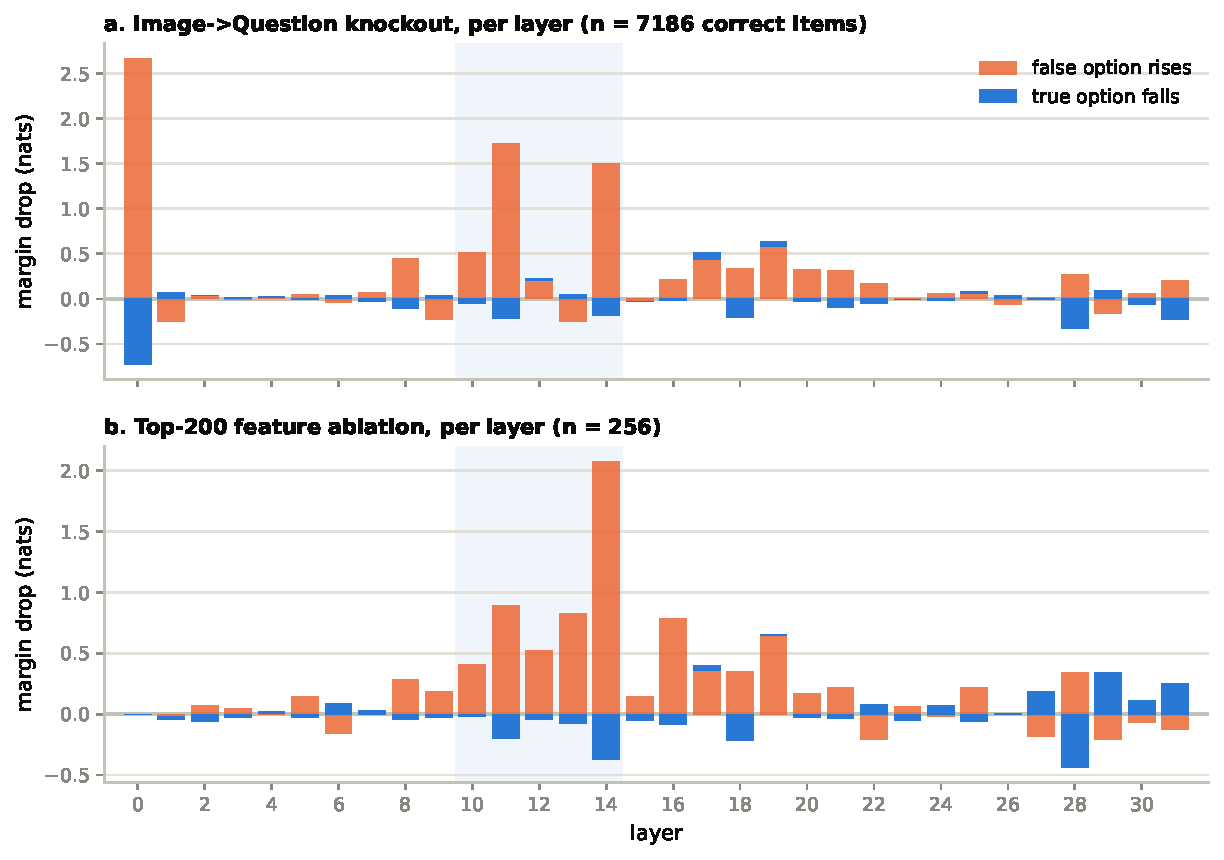
\includegraphics[width=\textwidth]{llava16_fig_decomposition}
  \caption{\textbf{What the margin drop is made of.} Per-layer margin drop split
  into the true option's loss (blue) and the false option's rise (orange), for
  Image$\rightarrow$Question knockout (a; $n = 7{,}186$) and top-200 feature
  ablation (b; $n = 256$). Both interventions are dominated by the false
  option's rise on this model, which is why their ratio compares like with
  like.}
  \label{fig:llava16-decomp}
\end{figure}

\begin{figure}[h]
  \centering
  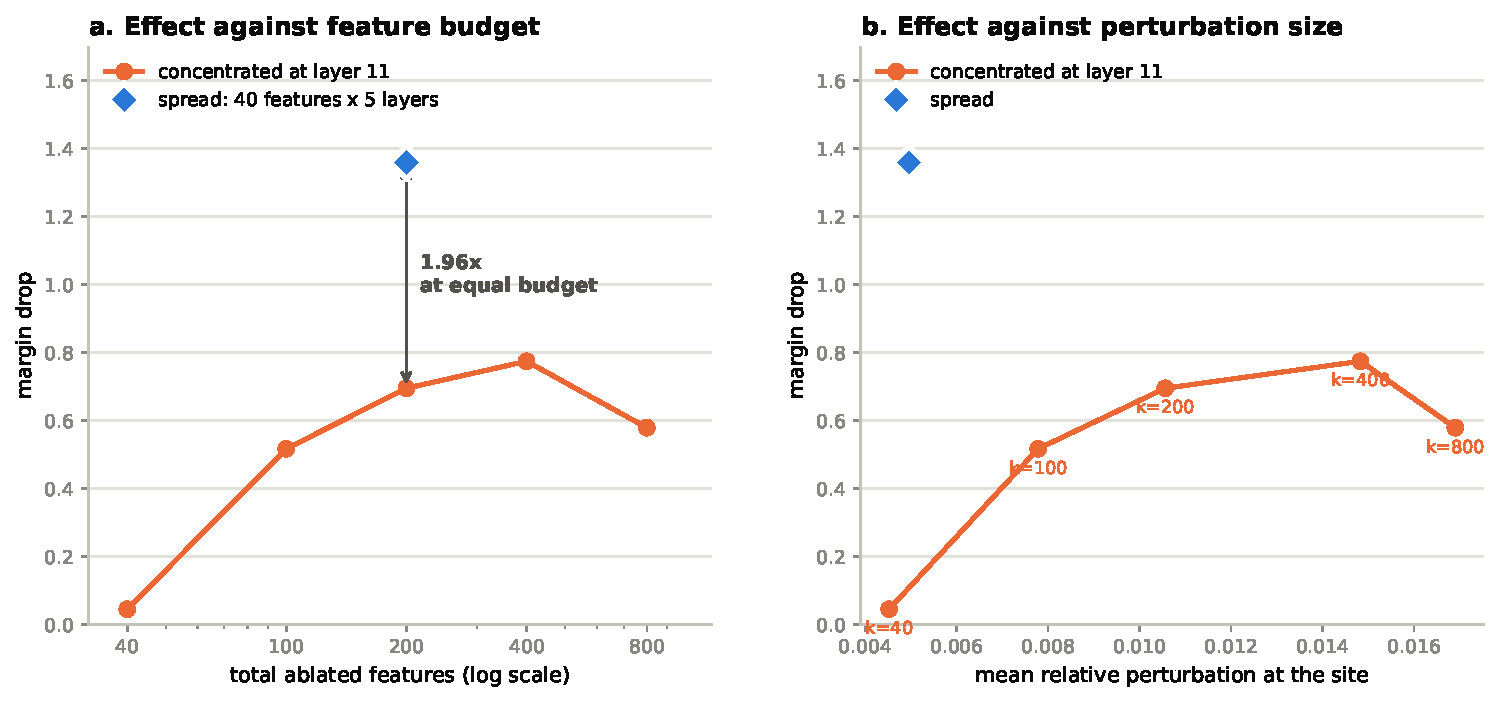
\includegraphics[width=\textwidth]{llava16_fig6_budget_distribution}
  \caption{\textbf{Budget and allocation on LLaVA-1.6.} (a) Margin drop against
  total ablated features for a budget concentrated at layer 11 ($k = 40$--$800$)
  and spread across layers 10--14 (40 per layer). (b) The same against the mean
  relative perturbation of the site. As on LLaVA-1.5 the concentrated curve is
  close to flat while the spread point at equal budget is far above it, by a
  factor of 1.96 against roughly three.}
  \label{fig:llava16-budget}
\end{figure}

\begin{figure}[h]
  \centering
  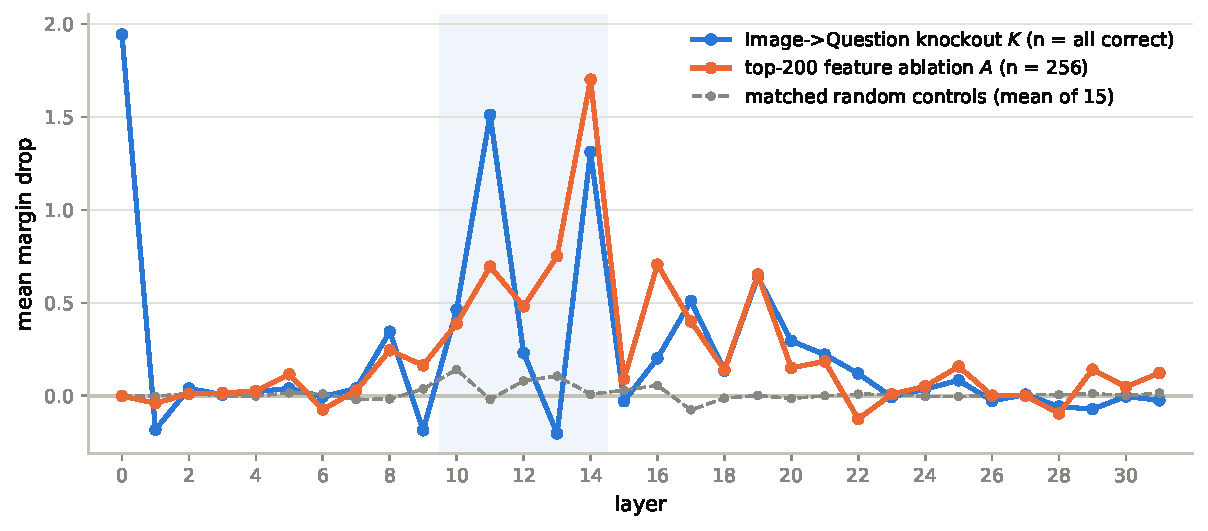
\includegraphics[width=\textwidth]{llava16_fig_single_layer}
  \caption{Top-200 \texttt{replace}-mode feature ablation at each of the 32
  layers ($n = 256$) with the mean of 15 activation-matched random controls, and
  the Image$\rightarrow$Question knockout for comparison.}
  \label{fig:llava16-single}
\end{figure}

\begin{figure}[h]
  \centering
  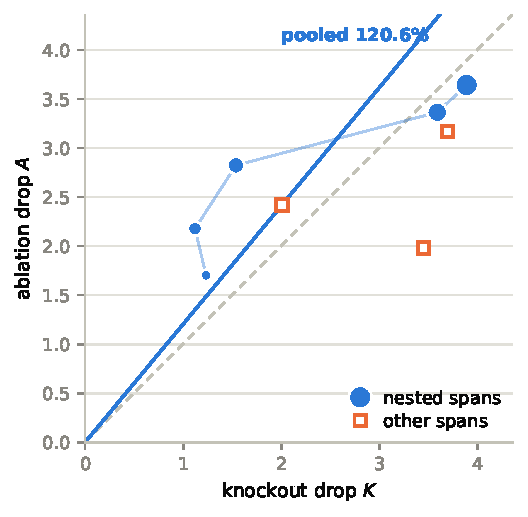
\includegraphics[width=0.58\textwidth]{llava16_fig8a_ablation_vs_knockout}
  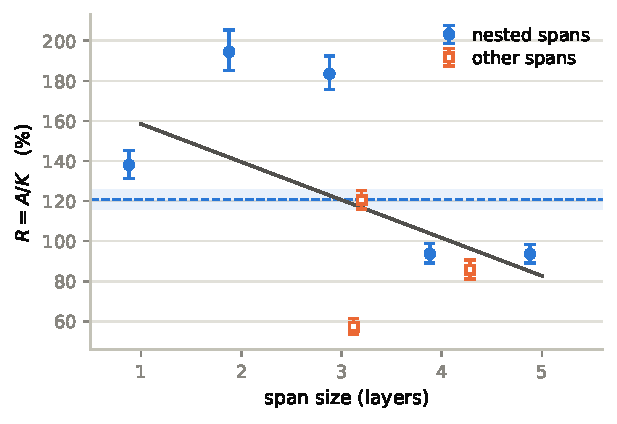
\includegraphics[width=0.66\textwidth]{llava16_fig8b_recovered_share}
  \caption{The LLaVA-1.5 span figures (Figures~\ref{fig:scaling}
  and~\ref{fig:rshare}) redrawn for LLaVA-1.6. Short spans lie above parity and
  wide ones just below it, and $R$ falls with span size ($-0.190$ per layer,
  95\% CI $[-0.212, -0.169]$) where the published run shows no trend
  ($-0.010$, $[-0.024, +0.003]$).}
  \label{fig:llava16-spans}
\end{figure}

\ifdefined\llavasixstandalone
  \bibliographystyle{plainnat}
  \bibliography{refs}
  \expandafter\enddocument
\fi

% ============================================================
% refs.bib additions -- ALREADY APPENDED to refs.bib; kept here for the record
% ============================================================
% @article{llava15,
%   title   = {Improved Baselines with Visual Instruction Tuning},
%   author  = {Liu, Haotian and Li, Chunyuan and Li, Yuheng and Lee, Yong Jae},
%   journal = {arXiv preprint arXiv:2310.03744},
%   year    = {2023}
% }
% @misc{llavanext,
%   title  = {{LLaVA-NeXT}: Improved reasoning, {OCR}, and world knowledge},
%   author = {Liu, Haotian and Li, Chunyuan and Li, Yuheng and Li, Bo and Zhang, Yuanhan and Shen, Sheng and Lee, Yong Jae},
%   year   = {2024},
%   month  = {January},
%   howpublished = {\url{https://llava-vl.github.io/blog/2024-01-30-llava-next/}}
% }
%
% ============================================================
% Suggested edits elsewhere in main_final.tex (for the author to apply)
% ============================================================
% Abstract, after the Gemma sentence suggested in gemma3_addition.tex: "A second
% replication on LLaVA-1.6, which keeps the same decoder, prompt, data and
% dictionary recipe and changes only the vision front-end, meets all three
% preconditions and still moves the recovered share from 72.6% to 93.6%, so the
% calibration is a property of the model together with its visual front-end
% rather than of the language model alone."
%
% Limitations paragraph: COMBINED replacement, superseding the one suggested in
% gemma3_addition.tex, since both edit the same sentence. Replace "Results come
% from one model, one synthetic task, one dictionary placement and one seed per
% layer" with "The positive results come from one model, one synthetic task, one
% dictionary placement and one seed per layer; the Gemma 3 replication
% (Section~\ref{sec:gemma}) shows what the same design returns when its
% preconditions fail, and does not establish that they can be met with
% pre-trained dictionaries, while the LLaVA-1.6 replication
% (Section~\ref{sec:llava16}) shows that meeting them does not make the
% recovered share reproduce across visual front-ends."
%
% Section 3.4 or the Discussion, where the 72.6% figure is introduced: consider
% adding "on this model and this visual front-end" -- Section~\ref{sec:llava16}
% gives 93.6% for the same decoder behind AnyRes tiling.
%
% Availability: the Gemma addition already points at
% https://github.com/KremerML/vlm-flow-probe; extend it to "the Gemma 3 and
% LLaVA-1.6 runs, adapters and configurations".
